%!TEX root = ../thesis.tex

\chapter{An introduction to the data: generic features of the Forum} \label{chap:introdata}

In the previous chapters, I described the context, theoretical background and potential approaches of a case study designed to understand longitudinal change in language use in \emph{\glslink{Forum}{Bipolar Forum}}, a \gls{bipolar} \gls{OSG}. In this and the next two chapters, I present the finding of the case study. The Bipolar Forum Corpus, and its Membership Stage Structure representing ten stages of membership, is the main dataset used. This chapter provides an introduction to the \gls{corpus} from both qualitative and quantitative perspectives. First, I present a genre analysis of a small selection of \glspl{post}, which highlights text structure beyond the level of the clause, and familiarises the reader with the kinds of language in the \gls{corpus}. This is followed by a presentation of shallow quantitative features in the \gls{corpus}' ten subcorpora. Chapter \ref{chap:interpersonal} contains findings from the \sctext{Mood} and \sctext{Modality} analysis. Chapter \ref{chap:experiential} contains findings from the \sctext{Transitivity} analysis.

%todo: tense?
%todo: copy edit
The case study was data\hyp{}driven and exploratory: results from one interrogation could largely determine what next needed to be explored. At other times, it was driven by the results of prior studies of language use in \glspl{OSG}, in communities generally, and in healthcare institutional settings. It was also theoretically informed, based on relationships between \gls{lexicogrammar} and meaning provided by \gls{SFL}. In this and the following two chapters, therefore, findings are generally accompanied by a brief discussion of their \gls{discourse-semantic} significance. There are two reasons for this structural choice. First, because the analysis was exploratory, with more delicate querying following broader querying, \glspl{discourse-semantic} needed to be presented \emph{in situ} in order to justify movement from one component of the \gls{lexicogrammar} to the next. Analysis of \glspl{discourse-semantic} was an integral part of the research process as it unfolded, rather than a task to be undertaken after the investigation had concluded. Second, the co\hyp{}presentation of wordings and their meanings more closely models the way humans use and understand language: it makes little sense to keep discussion of meaning separate from discussion of wording, as readers naturally interpret the meaning behind wordings as they encounter them.

Accompanying these chapters is a series of \texttt{Jupyter Notebooks}, containing the figures and concordance lines presented here, as well as the code used to generate them. They also document the functionality of \texttt{corpkit}, the toolkit used for analysis, in more detail, provide further examples from the auxiliary \glspl{corpus}, and document raw findings (i.e. frequency tables, etc.) that cannot be included in this chapter for reasons of space. The Notebooks are designed to facilitate reproducibility and transparency, and allow easy future applications of methods developed here to new datasets. They can be accessed via \texttt{GitHub} at \texttt{\href{https://github.com/interrogator/thesis}{https://github.com/interrogator/thesis}}.

\section{Genre and first contributions}

Though the case study analysis is for the most part a quantitative, computational one, the analysis begins with a qualitative, genre\hyp{}oriented analysis of some individual \glslink{post}{contributions} to the \gls{Forum}. I unpack generic features of a small selection of first \glspl{post} and replies they receive, using the approach to genre analysis outlined by \textcite{eggins_analysing_2004} and reviewed in Section \ref{sect:sfl}.
%This section is not intended to be an in-depth investigation of genre. Instead, it is intended to demonstrate that language choices in the community are affected by contextual parameters that are difficult to locate automatically. This is argued to be a major challenge of automatic discourse analysis in Chapters 7 and 8.
Foregrounding the qualitative analysis serves two main purposes. First, it provides a context for the abstracted \glslink{lexicogrammar}{lexicogrammatical} findings that follow: before analysing a \gls{corpus}, it makes sense for the researcher to have familiarised him\slash herself with some of its texts. Second, it foregrounds limitations inherent to the automated, computational searching of the \gls{corpus}. Contributions to the \gls{Forum} follow generic constraints---these, however, are not considered during automated searching. Later chapters discuss this problem, and potential solutions, in greater detail.

%todo: copy edit
One particular \gls{thread}, entitled `\textbf{am i bipolar and what should i do?}' is analysed in more detail than others. It is comprised of a new \glslink{member}{user}'s first \gls{post}, and replies from existing \glspl{member}. It was chosen because it contained \glspl{post} from \glslink{member}{users} spread across the ten stages of membership, and because it contained discussion of key social actors in the Field of discourse, such as friends and family and health professionals. Based on simple reading of \gls{Forum} \glspl{thread}, it also appeared to be relatively typical in terms of length, content and participating users.%
\endnote{The qualitative, generic analysis was in fact undertaken as a kind of pilot study, before any corpus linguistic analysis was performed. The \gls{thread} selected for analysis was therefore not chosen because it exemplified quantitatively identified features. The fact that many phenomena identified during the qualitative analysis are picked up during the \gls{corpus} analysis is not by design---rather, it highlights the surprising uniformity of texts within the genre of `first post threads'.}

\subsection{A user's first contribution to the Forum} \label{sect:jess-post}

% amylb1990400
On May 30, 2011, jessff1989787, a 20 year old female from England, \glslink{post}{posted} a new \gls{thread}, `\textbf{am i bipolar and what should i do?}', to the \glslink{Forum}{board}:

\begin{quote}
\resetlinenumber
\footnotesize{
\singlespacing{
\begin{linenumbers}
\begin{verbatim}
hi im jess new to this site, umm... well im currently 20 years 
old and have been diagnosed with depression from a young age 
but in the last 5 years or so i have been feeling very odd having 
some extreme highs which include loss of appetite concentration
using drugs and alcohol spending sprees and also sex, i can not 
control this when i get impulses like the above it is impossible 
though i have tried. I also suffer with depression which is quite
severe most of the time i find it hard to get out of bed or to 
even be able to connect with anyone including my partner who 
lives with me, i am hurting him so much but i dont feel like i 
can do anytjing about it
    i have asked my doctor to test me to see if i am bipolar as my 
antidepressants do not work even though they have been changed a 
million times!! he said no that he wont test me and i also asked 
for counselling and he also declined that, at the moment i feel 
that im loosing control of everything and its getting worse, i 
want to change my doctor and have been telling my partner i would 
but im scared of finding out that i am bipolar, but i really feel 
like either an extreme high or an extreme low is on the way and 
im quite scared i dont know what to do
    please help \end{verbatim}
\end{linenumbers}
}}
\end{quote}

The \gls{post} is reminiscent in form and function to \glspl{post} analysed in other work on \gls{OSG}: Jess indicates a need for general social support (\emph{im quite scared}, line 20) and requests advice (\emph{what should i do?}, title; \emph{i dont know what to do}, line 21). As noted by \textcite{smithson_developing_2012} and \textcite{varga2014grieving}, in order to legitimate herself as a potential \gls{member}, and add perlocutionary force to her request, Jess also offers a narrative designed to demonstrate that she likely suffers from \gls{bipolar}, and thus fulfills the membership criteria of the \glslink{Forum}{board}. Also notable is the sense of urgency, which has been conveyed through an apparent lack of planning within the post, spelling errors (\emph{anytjing}, line 11; \emph{loosing control}, line 17), and the pervasive joining of clauses through conjunction. As noted by \textcite{horne_doing_2009}, this may be a strategy for increasing the likelihood of response. In the context of bipolar disorder, it could also connote the onset of a manic episode, which would serve to bolster the claim to membership.

\subsubsection{Generic stages in Jess first post}

The \gls{post} appears to borrow from both \sctext{self\hyp{}introduction} and \sctext{narrative} genres identified by \textcite{labov_narrative_1997}. Indeed, in many ways, the \gls{post} conforms to the \sctext{narrative} genre, which has the structure:

\begin{quote}
(Abstract) $\hat{}$ Orientation $\hat{}$ Complication $\hat{}$ Evaluation $\hat{}$ Resolution $\hat{}$ (Coda)
\end{quote}

\noindent where

\begin{itemize}\onehalfspacing{
\item \sctext{Abstract} is an encapsulation of the point of the story
\item \sctext{Orientation} orients the listener to the circumstances of the story
\item \sctext{Complication} is temporally sequenced event which culminates in a problem
\item \sctext{Evaluation} is the attitude of the speaker toward the \sctext{complication}
\item \sctext{Resolution} is how the story's protagonist resolved the \sctext{complication}
\item \sctext{Coda} makes a point about the text and may reorient the listener to the present \cite[p.~32]{labov_narrative_1997}.
}
\end{itemize}
%
As shown in Table \ref{jess-genre}, the \sctext{abstract} stage is realised by the \gls{post}'s title; \sctext{orientation}, \sctext{complication} and \sctext{evaluation} do follow, though they appear to be recursive. Also different is the focus of the \sctext{evaluation}: here, it refers to an \sctext{evaluation} of the previous complication, rather than an evaluation of the narrative itself. The most significant deviation is that rather than a \sctext{resolution} (and optional \sctext{coda}), there is a \sctext{request} to other members for `help', presumably with the questions \glslink{post}{posted} in the title: whether or not she is bipolar, and how she should respond to her presented self\hyp{}evaluation.

\begin{table}[htb]\centering\small
\begin{tabularx}{\textwidth}{lX}

\toprule
Genre stage  & Sentences in Jess's first \gls{post}   \\ \midrule
\sctext{Abstract }    & am i bipolar and what should i do? \\ 
\sctext{Salutation}   & hi im jess   \\ 
\sctext{Orientation}  & (I am) new to this site,  umm... well im currently 20 years old and (I) have been diagnosed with depression from a young age but \\ 
\sctext{Complication (1)} & in the last 5 years or so i have been feeling very odd, (I have been) having some extreme highs which include loss of appetite concentration using drugs and alcohol spending sprees and also sex, \\ 
\sctext{Evaluation (1)}   & i can not control this when i get impulses like the above it is impossible though i have tried \\ 
\sctext{Complication (2)} & I also suffer with depression which is quite severe most of the time i find it hard to get out of bed or to even be able to connect with anyone including my partner who lives with me,   \\ 
\sctext{Evaluation (2)}   &  i am hurting him so much but i dont feel like i can do anytjing about it   \\ 
\sctext{Complication (3)} & i have asked my doctor to test me to see if i am bipolar as my antidepressants do not work even though they have been changed a million times!! he said no that he wont test me and i also asked for counselling and he also declined that, \\ 
\sctext{Evaluation (3)} & at the moment i feel that im loosing control of everything and its getting worse, \\ 
\sctext{Complication (4)} &  i want to change my doctor and (I) have been telling my partner i would but im scared of finding out that i am bipolar, but  \\ 
\sctext{Evaluation (4)}   & i really feel like either an extreme high or an extreme low is on the way and im quite scared i dont know what to do  \\ 
\sctext{Request}     & please help   \\ \bottomrule
\end{tabularx}
\caption{Genre stages in Jess's post}
\label{jess-genre}
\end{table}
%
Within a possible `first\hyp{}\gls{post} genre', explicit \sctext{Requests} are potentially optional \cite{vayreda_social_2009}, though other members may interpret descriptions of problems and the act of posting themselves as warranting the provision of advice \cite{goldsmith2000soliciting}. Some researchers \cite[e.g. ][]{herring_two_1996,weber_missed_2011} have noted that \glslink{member}{users} may not begin introductions to online communities with an explicit \sctext{salutation}: as all messages are attributed to the writer's username multimodally, and even new \glslink{member}{users} are likely familiar with the way in which the site presents \glspl{post}, \sctext{salutation}, if not rendered explicitly in prose, is in some sense embedded within the architecture of the \gls{forum} \gls{mode} itself. Given that all \glspl{post} must be titled, and that titles almost always summarise the content of the \gls{post}, \sctext{Abstract} is an obligatory stage. The generic structure provided by \textcite{labov_narrative_1997} could thus be adapted for this case as:

\begin{quotation}\small
\noindent Abstract $\hat{}$ Salutation $\hat{}$ Orientation $\hat{}$ [ Complication $\hat{}$ Evaluation ]\textsuperscript{n} $\hat{}$ (Request)
\end{quotation}
%
To characterise the extent to which Jess's post was representative of the genre, the two first \glspl{post} with the smallest wordcount were located and a basic genre stage analysis was performed (Table \ref{tab:two-genre-stage-analyses}). It was assumed that small first \glspl{post} would contain only obligatory genre features. These short \glspl{post} indicate that \sctext{evaluation} is an optional stage, and confirm that recursion of \sctext{complication} and \sctext{evaluation} is optional (though perhaps a key feature in developing a sense of urgency). \emph{Short Post B} shows that the optional \sctext{coda} noted by \textcite{labov_narrative_1997} appears to be possible within the first\hyp{}\gls{post} genre. This leaves a finalised generic structure for \gls{thread}\hyp{}initial first \glspl{post} within the \glslink{Forum}{Bipolar Forum}:

\begin{quotation}\small
\noindent Abstract $\hat{}$ Salutation $\hat{}$ Orientation $\hat{}$ [ Complication $\hat{}$ (Evaluation) ]\textsuperscript{n} $\hat{}$ (Request) $\hat{}$ (Coda)
\end{quotation}

\begin{table}[htb]
\small\centering
\begin{tabularx}{\textwidth}{lXX}
\toprule
Genre stage  & Sentences in Short Post A  & Sentences in Short Post B \\ \midrule
\sctext{Abstract}     & \emph{Lamictal}  & \emph{Depakote and hair thinning - any suggestions?}  \\
\sctext{Salutation}   & Hi-                                                                              & Hi                                                                      \\
\sctext{Orientation}  & I'm on my 3rd day of Lamictal and                                                & My daughter has been on Depakote for 4 months and                       \\
\sctext{Complication} & it's giving me weird almost headache like pains in my head                       & (she) has experienced some (h)air thinning                              \\
\sctext{Evaluation}   & ~                                                                                & ~                                                                       \\
\sctext{Request }     & Has anyone else had this happen while taking lamictal and when does it go away? & Has anyone out there found an effective way to counteract this problem? \\
\sctext{Coda}         & ~                                                                                & She is on 500mg per day. Any suggestions really appreciated.            \\
\bottomrule
\end{tabularx}
\caption{Genre stages in short first contributions}
\label{tab:two-genre-stage-analyses}
\end{table}
%
It is not enough, however, to simply look at the features of the \gls{post}: as \textcite{eggins_analysing_2004} explain, perhaps the best indicator of genre conformity is the way in which other members respond to the presented text. Thus, at this point, the investigation turns to consider replies to Jess's first \gls{post}.

\subsection{Replies to a first post}

Jess's first \glslink{post}{contribution} received six replies over the course of seven hours, from \glspl{member} with post counts ranging from five to over 5,000. Due to limitations of scope, only two of these replies have been selected for further analysis. They were selected based on the post count of the writer at the time of posting: one is a newer user (Subcorpus 03) and the other is a very senior member (Subcorpus 10). They also bookend the replies: the newer user is the first to respond to Jess, and the veteran member the last. The qualitative analysis, therefore, provides a description of language use at multiple stages of the membership course. The complete \gls{thread}, including the other four replies, is available in Appendix \ref{appendix:thread}.

The first reply was a response from \emph{Luvsoccer}, who had a total of five \glspl{post} to the \glslink{Forum}{board}:

\begin{quote}
\resetlinenumber
\footnotesize{
\singlespacing{
\begin{linenumbers}
\begin{verbatim}
It sounds like you might have bipolar to me. You need to change 
Drs. One with more knowledge apparently. The reason the 
antidepessants are not Working is because If you are bi polar 
and they put U on an antidepressant alone it can make things 
worse... I know from experience. Don't be scared it's treatable. 
Find you a dr that can make a correct Diagnosis and go from there. 
Good luck! \end{verbatim}
\end{linenumbers}
}}
\end{quote}
%
\noindent Following \emph{Luvsoccer} were four replies from other \glspl{member} at differing membership stages, unanalysed here. The final \gls{post} in the \gls{thread} was by \emph{Emz45}, who at the time of data collection had authored 5071 \glspl{post}:

\begin{quote}
\resetlinenumber
\footnotesize{
\singlespacing{
\begin{linenumbers}
\begin{verbatim}
Hi, welcome to the boards, hopefully we can help you out and be 
a support system for you. First off you're not A bipolar, *l* 
we're not things, it's a condition. From what you say, if 
sounds very likely that you might have Bipolar disoder. I would 
go to a psychiatrist for testing and find out. You don't have to 
have your docs permission to do this. If you're already seeing a 
psychiatrist and that's who's doing all the denying, then find a 
different one, because he's not doing his job, nor is he 
considering your best interest. That's all that you can really 
do in the beginning, find out what's what. We aren't docs here 
and can't diagnose you. But I think it would definitely be smart 
to go and get a diagnoses.

Take care, and please keep in touch, let us know how you're 
doing, okay?

Emz \end{verbatim}
\end{linenumbers}
}}
\end{quote}
%
\noindent The original poster did not contribute to the \gls{thread} again, but \glslink{post}{posted} to the \glslink{Forum}{board} on three other occasions in the next week, interacting again with \emph{Emz45}.

\subsubsection{Analysis of replies} \label{sect:qual-reply-analysis}

A first notable feature of the replies is their functional similarity. Both Luvsoccer and Emz45 offer social support (\emph{Don't be scared}, line 5; \emph{take care}, line 14), and encourage Jess to find a new doctor. Both also hint at a likely diagnosis based on the symptoms she has presented. In both cases, key ideological tenets of the \gls{Forum} are represented delicately. Both disparage the work of Jess's current psychiatrist (\emph{One with more knowledge}, line 2; \emph{he's not doing his job}, line 8). Both navigate the \gls{Forum}'s conflict between an inability to provide official diagnoses and an orientation toward supporting those who appear to have \gls{bipolar}. In fact, both provide near\hyp{}identical wordings:

\begin{enumerate}
\item \emph{It sounds like you might have bipolar to me}
\item \emph{From what you say, if sounds very likely that you might have Bipolar disoder}
\end{enumerate}
%
Both statements essentially amount to a lay diagnoses, with modulation, modalisation, embedding and dummy Subjects used to reduce certainty and to avoid attribution of the diagnosis to the speaker herself. Both further hedge the lay diagnosis by stressing the need for a professional diagnosis, and, in doing so, deny that what they offered was any kind of diagnosis at all.

%todo: first sentence doesn't make sense
The relationship between first\hyp{}\gls{post} and reply differ across the hierarchy of stratification. At the stratum of genre, unlike first \glspl{post}, the two replies do not conform rigourously to an identifiable sequence of clause functions. At the same time, the fact that the two responses overlap in content may be a useful indication that first \glspl{post} do constitute a genre that is recognised by other \glspl{member} of the \glslink{Forum}{community}. In terms of register, while the dimension of Field remains largely consistent (aside from Emz's avoidance of the topic of specific medications), the most dramatic differences are within Tenor: Jess is a prototypical newcomer, describing a medical history and current problem, positioning herself as vulnerable, lacking agency, and unable to participate effectively in her own care. In contrast, to Jess's descriptions of the past and present, Luvsoccer and Emz offer explanations and potential actions for the future. 

Within the \gls{lexicogrammar}, we can see differences in how the first and non\hyp{}first\hyp{}\glspl{post} construe reality via the system of \sctext{Transitivity}. All participants position themselves as Sensers, but the kinds of mental processes vary in their representation of subjectivity, reasoning and control. Jess characterised herself through subjective mental processes over which she has no agency (\emph{i have been feeling very odd}, \emph{i dont feel like i  can do anytjing about it}, \emph{i feel that im loosing control of everything}, \emph{i really feel like either an extreme high or an extreme low is on the way}); Luvsoccer, in contrast, \emph{know[s] from experience}, while Emz \emph{thinks} that diagnosis is the most important next step. Jess construes the health professional as an Agent, and most often, a Sayer (\emph{He said no}; \emph{He also declined that}), whose actions negatively affect her ability to obtain needed treatment. This contrasts with the other members, who reformulate health professionals as Goals (\emph{You need to change Drs}; \emph{Find you a dr}; \emph{I would go to a psychiatrist for testing}, etc.) Jess positions her partner, on the other hand, only as a Goal or Target, and never a Participant that puts processes in motion (\emph{i find it hard to [...] to connect with anyone including my partner}; \emph{i am hurting him so much}; \emph{I ... have been telling my partner}). For this reason, the partner is not construed at all in either response.

%Emz's advice provision strategy is to use modalisd material processes to show Jess the result of her reasoning: in \emph{I would go to a psychiatrist for testing and find out}, Emz foregrounds actions based on her familiarity with the situation.

There are also differences in the way first and non\hyp{}first \glspl{post} instantiate the system of \sctext{Mood}. All of Jess's major Mood choices are declarative and congruently work to provide information, until a final imperative, \emph{please help}, which shifts the function of the \gls{post} from the recursive narrative stages of \sctext{Orientation}, \sctext{Complication} and \sctext{Evaluation}, making a modulated demand on readers to address her declared fear and need for information (\emph{im quite scared i dont know what to do}). The Subject of most of Jess's clauses is \emph{I}, emphasising the self as the one invested with modal responsibility, and thus, the one who will honour any advice that others choose to provide. Modalisation of the self as Subject is used to stress an inability to modify behaviour (\emph{I can not control this}, \emph{I don't feel like I can do anything about it}). This is in contrast to the responses, which use interrogative and imperative Moods to request further information and to command the new user to respond. \emph{You} is by far the the most common Subject in the two replies, as the responses keep modal responsibility on Jess herself. Modalised declarative choices, meanwhile, do not always provide information, but may also issue directives in the form of advice: Emz does this twice, casting herself as the hypothetical actor in the first (\emph{I would go to a psychiatrist for testing and find out}) and using rank\hyp{}shifted and non\hyp{}rank\hyp{}shifted modulation strategies to hedge the second (\emph{\textbf{I think} it would \textbf{definitely} be smart to go and get a diagnoses}).

%todo: repeated
Also observable are subtle differences between the two replies, caused primarily by membership stage. As mentioned earlier, Luvsoccer's \gls{post} is a part of Subcorpus 03; Emz45's is in Subcorpus 10. First, in terms of choices of Field, Luvsoccer attempts to explain the reason that antidepressants are not helping, while Emz avoids the topic completely. This is related to the gradual rise in general offerings of social support and the decrease in references to specific medications \cite{wang_stay_2012}: veteran \glslink{member}{users} may refrain from offering specific advice on medication choice and dosage, as within a normative biomedical ideology, these are domains restricted to the health professional \cite{vayreda_social_2009}. Another key difference between the two replies is in the source of knowledge underlying the advice. Luvsoccer foregrounds personal experience by construing herself as the Senser (\emph{It sounds to me}; \emph{I know from experience}); Emz, on the other hand, only represents herself as a \gls{member} of the \glslink{Forum}{board} (\emph{hopefully we can help you}, \emph{we aren't docs and [we] can't diagnose you}), as the Subject within hypothetical advice (\emph{I would go to a psychiatrist}), and within rank\hyp{}shifted modulation of another advice instance (\emph{I think it would definitely be smart to go and get a diagnoses}). 

A third notable difference is in the ways the two replies are concluded. After offering advice, Luvsoccer simply writes \emph{Good luck!}, effectively signalling the end of her part in the interaction. Emz, on the other hand, attempts to maintain dialogue (\emph{please keep in touch, let us know how you're 
doing, okay?}) by commanding the user to report back, hedging through the use of a tag question seeking agreement\slash permission. Emz's conclusion opens up space for further exchange within a community where all interpersonal exchange is understood to contribute to wellbeing \parencite[c.f.][]{althoff_counseling_2016}.\endnote{This can also be seen as an attempt to maintain active discussion within the forum more generally: veteran members contribute by choice, and are therefore personally invested in the health of the community itself.}

Emz45's reply also shows us that veterans' preference for jargonisation (see Chapter \ref{chap:experiential}) is not absolute. Here, presumably because she is interacting with a new \glslink{member}{user}, she opts for lay terms (\emph{bipolar disoder}, \emph{psychiatrist}, \emph{diagnoses}). This contrasts with Luvsoccer, who uses the developing shorthand forms for health professionals (\emph{dr}, \emph{drs}), but not the jargonised variants that distinguish between particular kinds of health professional.

A final important difference between the two replies is the way in which they advocate changing doctors\slash psychiatrists. Compare:

\begin{multicols}{2}
\begin{quote}
\sctext{Luvsoccer}

\emph{You need to change Drs. One with more knowledge apparently.} ~\\~\\~\\
\end{quote}

\begin{quote}
\sctext{Emz45}

\emph{If you're already seeing a psychiatrist and that's who's doing all the denying, then find a different one, because he's not doing his job, nor is he considering your best interest}
\end{quote}
\end{multicols}
%
\noindent Though Emz is by far the more senior member, her advice is conditional, and sensitive to an ambiguity concerning the type of health professional Jess is currently seeing. Emz is also the only one who provides an explicit reason for the need to change. Luvsoccer's reasoning must be inferred from the statement that the doctor lacks knowledge, and has prescribed what she believes to be inappropriate medication. 

%Notably, Luvsoccer's reply is ignored by Emz, despite a great deal of overlap in content. This too hints at the generic nature of first \glslink{post}{contributions}: unlike non-first\hyp{}\gls{post} threads, first \glspl{post} are not many-to-many discussions, but one-to-many narratives that seek one-to-one responses.

%Advice is dispensed throughout Lurvunning's reply, with imperative moods used to explicitly command the user to not be scared, and to find a new doctor. Advice is

The similarities and differences between the two replies highlight the way in which expertise and social status develop over the course of membership. It takes only a handful of prior \glslink{post}{contributions} to the \glslink{Forum}{board} to adopt the role of the expert when interacting with a newcomer. Imperatives and jargonised lexis are used to reinforce this role in earlier stages of membership. What may take time to develop are the subtle routines for providing information and support while maintaining an inclusive, non\hyp{}hierarchical space. The main point of contrast between the two replies is that Luvsoccer's style is terse, lacking almost entirely in elaborations and pleasantries, while Emz disperses similar health information and advice within a text that is rich in incongruence and modulation, with the ultimate aim of establishing rapport. This phenomenon will be shown quantitatively in the following two chapters.

What remains, at this point, is to demonstrate the extent to which the \gls{thread} analysed here is prototypical of the \gls{Forum}'s contents as a whole. More specifically, the remainder of this chapter, as well as the next two chapters, chart language choices quantitatively over ten stages of membership. It is useful to remember that Jess's first \gls{post} is a part of the first subcorpus, Luvsoccer's reply is in the third, and Emz's in the 10th and final subcorpus, for all 560th \glspl{post} or above.

\section{Shallow lexicogrammatical features} 

The first quantitative part of the case study involves a short analysis of shallow features of the \glspl{corpus}, derived from subcorpus features such as word count, clause count, and the distribution of word classes\slash \gls{POS} tags. Features analysed here are only very general approximates of register, crossing metafunctional lines and ignoring the entire dimension of lexis.

A secondary purpose for general frequency counting is for use in relative frequency calculation in the following two chapters. Rather than discovering the frequency of a given verb compared to all words in the dataset, it is more instructive to compare the verb to all verbs, or all processes of a given type. In this way, analysis remains sensitive to broader grammatical changes that occur throughout membership: if texts become more highly nominalised, when comparing frequencies with all words in the dataset, a particular noun may seem to increase in frequency, when in reality, it is less and less often chosen ahead of other related nouns.

%The P (Postcount) corpus is the main dataset investigated. It contains ten subcorpora, representing \glspl{post} made at ten stages of membership.

\begin{figure}[htb]
\centering
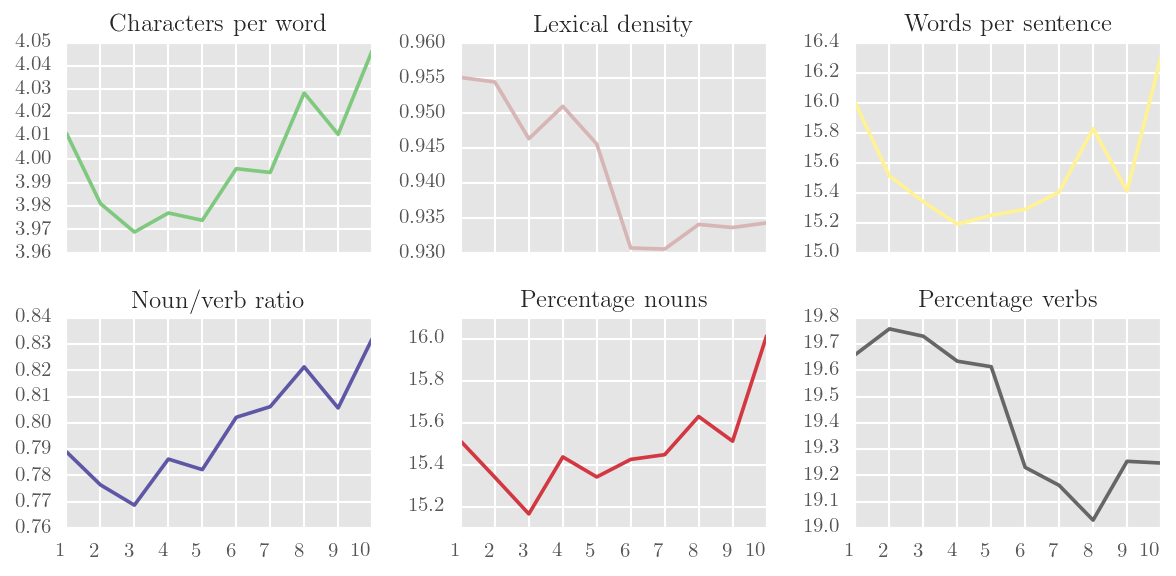
\includegraphics[width=\textwidth]{../images/derived-shallow-features-in-p-corpus.png}
\caption{Derived shallow features for the Membership Stage Structure}
\label{fig:derived_shallow_P}
\end{figure}

A number of features exhibit relatively consistent longitudinal change (see Figure \ref{fig:derived_shallow_P}). Many of these features point toward an increasingly `scientised' register \cite{harvey_disclosures_2012}, such as nominalisation and word length, which are related, as nominalisation typically involves the addition of derivational morphemes to non\hyp{}nominals \cite{simon-vandenbergen_grammatical_2003}. In the same vein, verbs become less frequent over time. That said, \emph{noun} and \emph{verb} are formal categories that can only approximate semantic notions of \emph{Things} and \emph{Events}, or, at a higher rank, \emph{Participants} and \emph{Processes}. More attention will be paid to these in the chapters that follow.

%\begin{figure}[htb]
%\centering
%\includegraphics[width=0.7\textwidth]{../images/firstpost-example.png}
%\caption{A first post example, featuring a medical history narrative}
%\label{fig:firstpost-example}
%\end{figure}

Another trend visible in Figure \ref{fig:derived_shallow_P} is that the first subcorpus---that is, first \glspl{post} to the \gls{Forum}---has features that often differ from the overall upward or downward trend. Lexical density (defined here as the ratio of lexical words to clauses) is one example: peaking in first \glspl{post}, it remains relatively stable thereafter. First \glspl{post} also deviate from general trends in terms of average character per word, words per sentence, noun\slash verb ratio, and the relative frequency of nouns in general. These features indicate that first \glspl{post} are considerably more packed with content than later contributions. Higher lexical density in first \glspl{post} is to be expected: \glslink{member}{users} are under no time constraints, as they are not responding to an interlocutor, and because other \glspl{member} are not aware that a message is being prepared. At the same time, users' initial contributions are more formal because it is in these contributions that new \glspl{member} first make interpersonal demands (solicitation of responses) on other \glspl{member}, who are by definition more senior figures in the community. Many \glslink{member}{users} may also have longer\hyp{}term considerations in mind: their first \glspl{post} constitute an initial bid for acceptance by the \glslink{Forum}{community}, and thus are tailored to conform to others' expectations of politeness. After the user is welcomed into the \glslink{Forum}{community}, lexical density quickly stabilises, and many other features begin a stable trajectory. These are early quantitative indications of a difference between the first and non-first \glspl{post} at the strata of \emph{genre} and \emph{register}. This discussion will be picked up in Chapter \ref{chap:discuss-bp}, following the presentation of findings from more delicate querying of the \gls{lexicogrammar} in Chapters \ref{chap:interpersonal} and \ref{chap:experiential}.

\section{Controlling for self-selection bias}

The Membership Stage Structure has the potential for self-selection bias: \glslink{member}{users} who become veterans may use language differently even in their first \glslink{post}{contributions}. To control for this, the Future Veteran Structure (which contains no \glspl{post} from early dropouts) and the Comparative Structure (which has subcorpora for Dropouts and Future Veterans) can be used. In the section below, I briefly demonstrate that the language use of those \glslink{member}{users} who progress to veteran stages is not quantitatively different from the language of \glslink{member}{users} who drop out during early \glslink{post}{contributions}. The implication of this finding is that future veteran members' language choices do in fact change in predictable ways over time.

% I perform a limited number of investigations of these two \glspl{corpus}, in order to

\subsection{Future Veteran Structure}

The Future Veteran Structure contains no \glspl{post} from \glspl{member} who dropped out before contributing 30 times. It is structured identically to the Membership Stage Structure. When using this \gls{corpus}, the first four stages of membership are collapsed into a single stage, in order to make sure that each subcorpus contains a quantifiably reliable amount of text.

%\begin{table}
%\centering
%\small
%\begin{tabular}{lrrrrrrr}
%\toprule
%{} &    Verb &    Noun &  Pronoun &  Preposition &  Adverb &  Determiner &  Adjective  \\
%\midrule
%01 &   13491 &   10387 &     8236 &         6432 &    5126 &        4297 &       4229  \\
%02 &   20555 &   16320 &    12919 &         9834 &    7989 &        6679 &       6347  \\
%03 &   36500 &   28904 &    23048 &        17425 &   14048 &       11805 &      11328  \\
%04 &   71660 &   56816 &    45953 &        34037 &   27859 &       23313 &      21867  \\
%05 &  134443 &  105099 &    86145 &        63164 &   51718 &       43531 &      40638  \\
%06 &  178530 &  143212 &   114036 &        84616 &   69463 &       59305 &      55074  \\
%07 &  172483 &  139058 &   110574 &        81344 &   67335 &       57616 &      53652  \\
%08 &  185094 &  152034 &   117622 &        90276 &   72004 &       62675 &      59043  \\
%09 &  161888 &  130437 &   102969 &        78575 &   62341 &       55102 &      49909  \\
%10 &  156886 &  130532 &    99547 &        81309 &   56942 &       55112 &      48051  \\
%\bottomrule
%\end{tabular}
%\caption{Word classes in V Corpus}
%\label{tab:wc_V}
%\end{table}

\begin{figure}[htb]
\centering
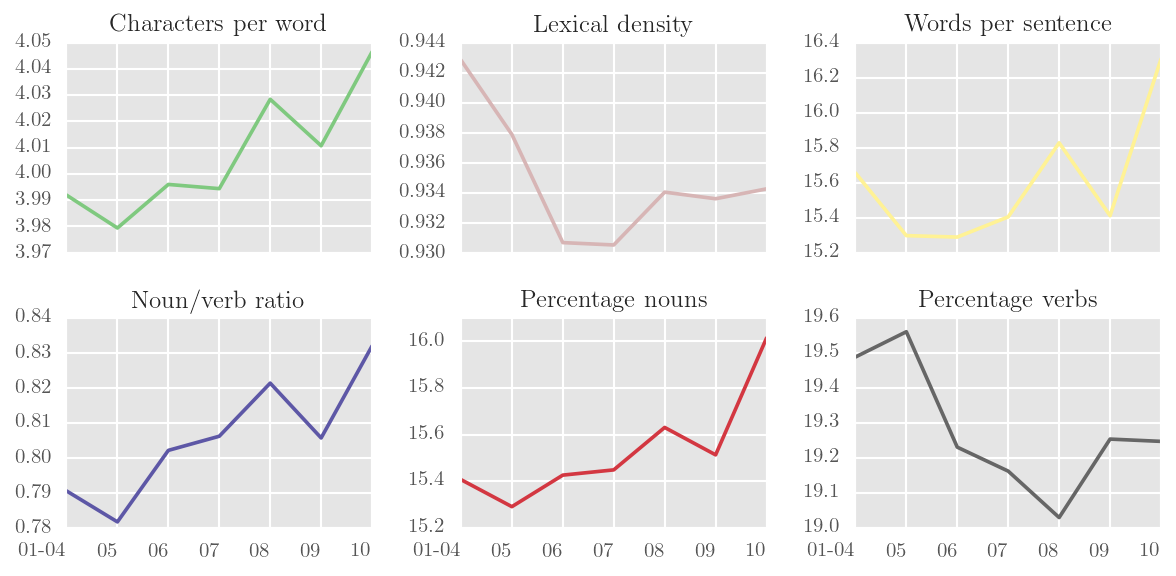
\includegraphics[width=\textwidth]{../images/derived-shallow-features-in-v-corpus.png}
\caption{Derived shallow features for the Future Veteran Structure}
\label{fig:derived_shallow_V}
\end{figure}

There is generally little difference from the Membership Stage Structure (compare with Figure \ref{fig:derived_shallow_P}), suggesting that future veteran \glslink{member}{users} use a similar register to non\hyp{}future \glspl{member} in early \glspl{post}.

\subsection{Comparative Structure}

Comparative Structure has two subcorpora: the first contains \glspl{post} from any \gls{member} who \glslink{post}{posted} fewer than 30 times; the second contains the \glspl{post} of members who \glslink{post}{posted} 30 or more times.

\begin{figure}[htb]
\centering
\includegraphics[width=0.6\textwidth]{../images/derived-shallow-features-in-C-corpus.png}
\caption{Derived shallow features for the Comparative Structure}
\label{fig:derived_shallow_C}
\end{figure}

Figure \ref{fig:derived_shallow_C} shows a great deal of similarity between the \glspl{post} of Dropouts and the early \glspl{post} of future Veterans. This means that broad register features change over the course of membership.

\section{Mapping membership stages to Forum history}

The Longitudinal Structure takes \glspl{thread} as the unit of analysis, rather than \glspl{post}. Each \gls{thread} is grouped by the year in which it was created, so that linguistic change across the \gls{Forum}'s history can be examined. This corpus contains speaker metadata, making it possible to track one or more specific speakers longitudinally.

%ntodo: figure missing

\begin{figure}[htb]
\centering
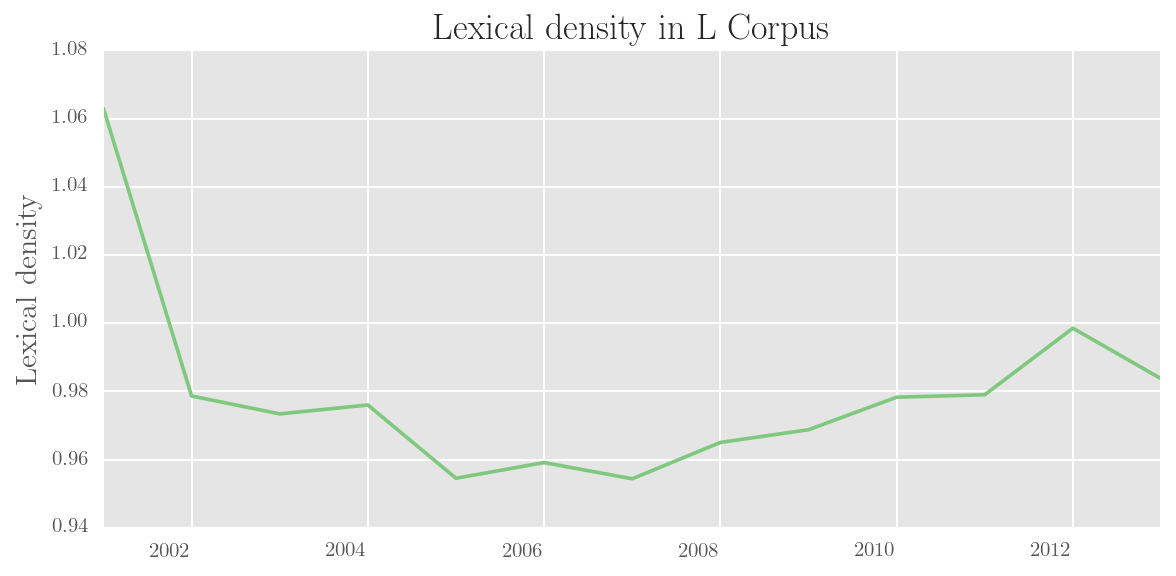
\includegraphics[width=0.6\textwidth]{../images/lexical-density-in-l-corpus.png}
\caption{Lexical density in the Longitudinal Structure}
\label{fig:lex_dens_L}
\end{figure}



Figure ?? shows that the Longitudinal Structure does not vary consistently in most shallow feature dimensions. One exception is in lexical density (Figure \ref{fig:lex_dens_L}), which steadily rises throughout much of the \gls{Forum}'s history---fluctuations observed in the first and last subcorpora could well be the result of chance (due to their smaller sample size---see Section \ref{sect:l-corpus}). That said, it is not impossible that the first ever contributions to a \gls{forum} adopt a slightly more formal tone, as users air on the side of (polite) caution until the normative linguistic practices of the community take shape. The finding also hints at phylogenesis change, where linguistic practices of one generation of users within the \gls{Forum} can have a lasting effect on the practices of the next \cite{danescu-niculescu-mizil_no_2013}.

Though limitations of scope prevent a larger analysis of the Longitudinal Structure, it provides preliminary support for the notion that veteran \glslink{member}{users} may have lasting change on the discursive orientation of an online community. In terms of methodology, it demonstrates the utility of dynamic subcorpus structures: the same data, differently organised, can be analysed with identical methods in order to answer a different set of research questions. The Longitudinal Structure allows observation of the relationship between language use and the passage of time. Given our knowledge that ideologies are embraced and abandoned within the community at different points in time, it is reasonable to hypothesise that the time at which a new user enters the community could have an effect on the values they represent in later stages of membership. 

\section{Chapter summary}

In this chapter, I have provided preliminary analysis of the Bipolar Forum Corpus from two opposite perspectives. First, I have approached three \glspl{post} within a single \gls{thread} from below, looking at realised words and wordings in sequence. This analysis highlighted differences in how Forum members use language over the course of membership, echoing in many respects existing findings in discourse-oriented \gls{OSG} literature: newcomers' first \glspl{post} may conform to a first\hyp{}\gls{post} genre in which medical histories and current problems are outlined, with the dual aim of both legitimating the self as a potential member and eliciting responses from readers.

Second, I have looked at the corpus from above, looking at broad changes in shallow grammatical features, without consideration of the role of lexis, or of the distinction between metafunctions. Findings here showed that some features vary in more or less consistent ways over the membership course, and may be related to overall shifts in the register of users as they progress toward veteran status within the community. What remains, however, is to fill in the middle ground between realised samples of text and broad grammatical features. This analysis, segmented by metafunction into \sctext{Mood} and \sctext{Transitivity} parts, is performed over the next two chapters.
